\section{Numerical experiments}
\label{Section: Numerical experiments}
We conduct extensive experiments to evaluate the effectiveness of DualHash against several state-of-the-art hashing methods on three
standard image retrieval datasets. All experiments use PyTorch 1.12.1 with CUDA 11.3 on an NVIDIA V100 GPU platform.
% Visualizations are implemented using Python on macOS 15.3.2. 
% % The codes are available at \red{\url{https://anonymous.4open.science/r/DualHash_NeurIPS}.}
\subsection{Experimental Setup}
\paragraph{Datasets} \textbf{CIFAR-10}\footnote{\url{https://www.cs.toronto.edu/~kriz/cifar.html}} is a \textbf{single-label} dataset comprising 60,000 $32 \times 32$ color images from 10 classes. 
In our experiment, we randomly sample 1,000 images per class (10,000 total) for training, 500 per class (5,000 total) for validation, and 500 per class (5,000 total) for testing.
\textbf{NUS-WIDE}\footnote{\url{http://lms.comp.nus.edu.sg/research/NUS-WIDE.htm}} is a \textbf{multi-label} dataset containing approximately 270,000 web images, each annotated with one or more labels from 81 categories. 
% Following \cite{liuHashingGraphs, laiSimultaneousFeatureLearning2015, liuDeepSupervisedHashing}.
In our experiment, we use a subset of 195,834 images from the 21 most frequent concepts (each with at least 5,000 images) and randomly sample 700 images per class (14,700 total) for training, 300 per class (6,300 total) for validation, and 300 per class (6,300 total) for testing.
\textbf{ImageNet}\footnote{\url{https://www.image-net.org/}} is a large-scale image dataset from the Large Scale Visual Recognition Challenge (ILSVRC 2015). It contains over 1.2 million images in the training set and 50K images in the validation set, where each image is \textbf{single-labeled} by one of the 1,000 categories. Following \cite{Cao2017HashNetDL}, in our experiment, we randomly select 100 categories to create ImageNet-100. We use 100 images per category (10,000 total) for training, 30 per category (3,000 total) for validation, and 50 per category (5,000 total) for testing. The training, validation, and testing sets are mutually exclusive with no data overlap.

% \vspace{3pt}
\paragraph{Training Setup}  It is worth noting that our method is compatible with different similarity measurement paradigms, including pointwise, pairwise and tripletwise methods. In our experiments, we focus on deep supervised pairwise hashing using a pairwise cross-entropy loss \( f \) and the nonsmooth W-type regularization term \( h(z) = \lambda \| |\bz| -1 \|_1 \). 

% \vspace{3pt}
\paragraph{Baselines} We compare against eight baselines: SDH \cite{shenSupervisedDiscreteHashing2015}; four deep hashing methods with W-type regularizations (DHN \cite{zhuDeepHashingNetwork2016}, DSH \cite{liuDeepSupervisedHashing}, DTSH \cite{wang2016DTSH}, MDSHC \cite{wang2023deep}); 
and three state-of-the-art methods addressing quantization error (HashNet \cite{Cao2017HashNetDL}, DSDH \cite{li2017deep}, OrthoHash \cite{hoeOneLossAll2021}). Following \cite{liuDeepSupervisedHashing}, we report the mean Average Precision (mAP), precision curves (P@topK), and precision within Hamming radius 2 (P@r=2). Detailed definitions and a full introduction of the baselines are provided in the Supplementary Materials A.

% \vspace{3pt}
\paragraph{Architecture} For fair comparison, all deep learning-based methods employ AlexNet and ResNet-50\footnote{AlexNet is the default backbone unless specified.} as the 
backbone network and use ELU activation to leverage its 
1-Lipschitz continuous gradient property for satisfying the smoothness assumption (\Cref{Ass: main assumptions}(ii)).
All images are resized to $256 \times 256$ pixels and center-cropped to 
$224 \times 224$. We fine-tune the pre-trained convolutional layers 
(conv1--conv5) and fully connected layers (fc6--fc7), while initializing 
any newly added layers with Kaiming initialization\footnote{Although DSDH \cite{li2017deep} uses the CNN-F architecture, it shares a similar structure with AlexNet—both consist of five convolutional layers followed by two fully connected layers.}.
For the non-deep method (SDH \cite{shenSupervisedDiscreteHashing2015}), we use the following input features: 512-dimensional GIST vectors for CIFAR-10, 500-dimensional bag-of-words features for NUS-WIDE, and 1024-dimensional CNN features for ImageNet-100. During training, we monitor validation performance in real-time to observe convergence behavior and adjust hyperparameters accordingly. For evaluation, we use the training set as the retrieval database and the test set as queries.
\begin{remark}{For standard ReLU-activated backbones, existing nonsmooth stochastic optimization literature establishes convergence guarantees for such networks under weaker tame or weakly convex frameworks \cite{davis2020stochastic,maiConvergenceStochasticGradient2020}, which are fundamentally distinct from our smooth primal-dual analysis. Extending our framework to this nonsmooth setting is an important direction for future work.}
\end{remark}

% \vspace{3pt}
\paragraph{Hyperparameter Settings} 
{Unless the original implementation imposes a method-specific component, all deep baselines are trained under the same data splits, evaluation protocol, backbone family, image preprocessing, and early-stopping rule as DualHash.} All models are trained for a maximum of 300 epochs with early stopping based on validation mAP. We use a fixed mini-batch size of 256 for CIFAR-10 and 128 for NUS-WIDE and ImageNet-100.
For DualHash-StoM, the learning rate $\eta_k$ is selected from $\{10^{-4}, 10^{-3}, 10^{-2}, 10^{-1}\}$ with step decay, approximating $\eta_k \sim O(L_F^{-1})$ without computing $L_F$. For DualHash-StoRM, $\eta_k$ is chosen from $\{5 \times 10^{-3}, 5 \times 10^{-2}, 5 \times 10^{-1}\}$ following $\mathcal{O}(T^{-1/3})$ scaling, and $\rho_k$ is selected from $\{0.01, 0.05, 0.1, 0.2, 0.7\}$ via cross-validation. For DualHash-StoM, we set the momentum parameters $\alpha_k = \beta_k = 0.905$. Baselines follow their official optimizer settings. The proximal operator for $h^*(\cdot)$ requires $\tau < \lambda$ to ensure well-defined updates. We tune $\lambda \in \{10^{-3}, 10^{-2}, 5\times 10^{-2}, 10^{-1}\}$ and set $\tau$ accordingly. For all datasets, we set $\tau = 10^{-2}$, $\lambda = 5 \times 10^{-2}$, and $\gamma = 3$. In our practical implementation, we use a dual-step-size variant for multipliers \(\bm{\Lambda}\), i.e., the \(\bm{\Lambda}\)-update uses step size \(0.1\tau\), while the theoretical analysis is stated for the unified \(\tau\)-scheme in \Cref{Section: Methodology,Section: Convergence analysis}. 
% All results represent averages over 10 independent runs. 
% \vspace{3pt}
\subsection{Convergence Validation}
\label{Subsection: Convergence validation and performance efficiency analysis}
\begin{table}[t]
    \centering
    \caption{The mAP results of DualHash and baselines with different numbers of bits on CIFAR-10 and NUS-WIDE datasets.}
    \label{Table: baselines mAP}
    \resizebox{\linewidth}{!}{
    % \begin{tabular}{1\textwidth}{@{\extracolsep{\fill}}ccccccccc@{}}
    \begin{tabular}{ccccccccc}
        \toprule
        \multirow{2}{*}{Methods} & \multicolumn{4}{c}{CIFAR-10 (mAP@All)} & \multicolumn{4}{c}{NUS-WIDE (mAP@5000)} \\
        \cmidrule(lr){2-5} \cmidrule(lr){6-9}
         & 16 bits & 32 bits & 48 bits & 64 bits & 16 bits & 32 bits & 48 bits & 64 bits \\
        \midrule
        SDH \cite{shenSupervisedDiscreteHashing2015} & 0.4254 & 0.4575 & 0.4751 & 0.4855 & 0.4756\textsuperscript{*} & 0.5545\textsuperscript{*} & 0.5786\textsuperscript{*} & 0.5812\textsuperscript{*} \\
        SDH-CNN & 0.6665 & 0.6501 & 0.6484 & 0.6260 & 0.4872 & 0.6529 & 0.6451 & 0.5239 \\
        DSH \cite{liuDeepSupervisedHashing} & 0.6610 & 0.7530 & 0.7817 & 0.8010 & 0.5195 & 0.6629 & 0.6617 & 0.6634 \\
        DTSH \cite{wang2016DTSH}  & 0.7661 & 0.7501 & 0.7651 & 0.7744 & 0.6590 & 0.6845 & 0.7130 & 0.7371 \\ 
        DHN \cite{zhuDeepHashingNetwork2016} & 0.6568 & 0.7608 & 0.7838 & 0.8051 & 0.5562 & 0.6427 & 0.6808 & 0.7042 \\
        HashNet \cite{Cao2017HashNetDL} & 0.3354 & 0.6511 & 0.7732 & 0.8396 & 0.5879 & 0.6769 & 0.7221 & 0.7249 \\
        DSDH \cite{li2017deep} & 0.2732 & 0.3648 & 0.4222 & 0.4941 & 0.5153 & 0.5953 & 0.6338 & 0.6619 \\
        OrthoHash \cite{hoeOneLossAll2021} & 0.8070 & 0.8059 & 0.8387 & 0.8355 & \textbf{0.6653} & 0.6912 & 0.7083 & 0.7176 \\
        MDSHC \cite{wang2023deep} & 0.8142 & 0.8238 & 0.8350 & 0.8262 & 0.5902 & 0.6452 & 0.6081 & 0.6493 \\
         \cmidrule(lr){2-9} 
        \textbf{DualHash-StoRM} & 0.8037 & 0.8051 & 0.8168 & 0.8345 & 0.6485 & 0.6802 & 0.6951 & 0.6982 \\
        \textbf{DualHash-StoM} & \textbf{0.8215} & \textbf{0.8481} & \textbf{0.8534} & \textbf{0.8539} & 0.6339 & \textbf{0.7002} & \textbf{0.7248} & \textbf{0.7448} \\
        \bottomrule
    \end{tabular}}
    \vspace{-2ex}
    \parbox{\linewidth}{\footnotesize
    \textsuperscript{*}SDH results on NUS-WIDE are cited from HashNet and reported for reference under a similar protocol.
    \textbf{Bold} values indicate the best results.
    }
\end{table}
\begin{figure}[t]
    % \vspace{-1mm}
    \centering
    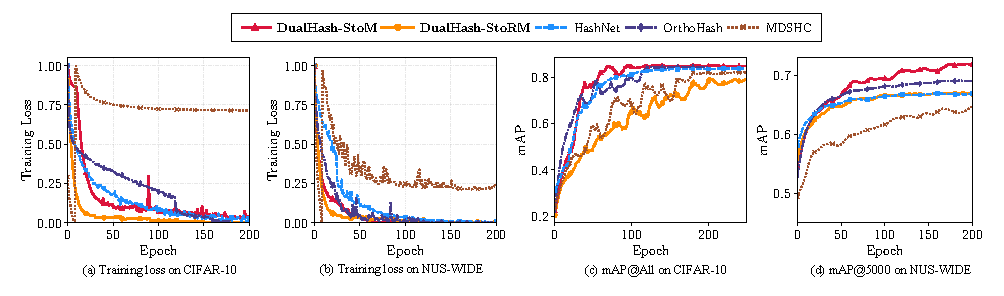
\includegraphics[width=0.95\linewidth]{results_images/ex1_4figures_new.pdf}
    \caption{Training loss and the mAP results of DualHash and baselines with 64 bits on CIFAR-10 and NUS-WIDE datasets.}
    \label{fig:training_loss_map_2datasets}
    \vspace{-2ex}
\end{figure}
\begin{figure}[t]
    % \vspace{-1mm}
    \centering
    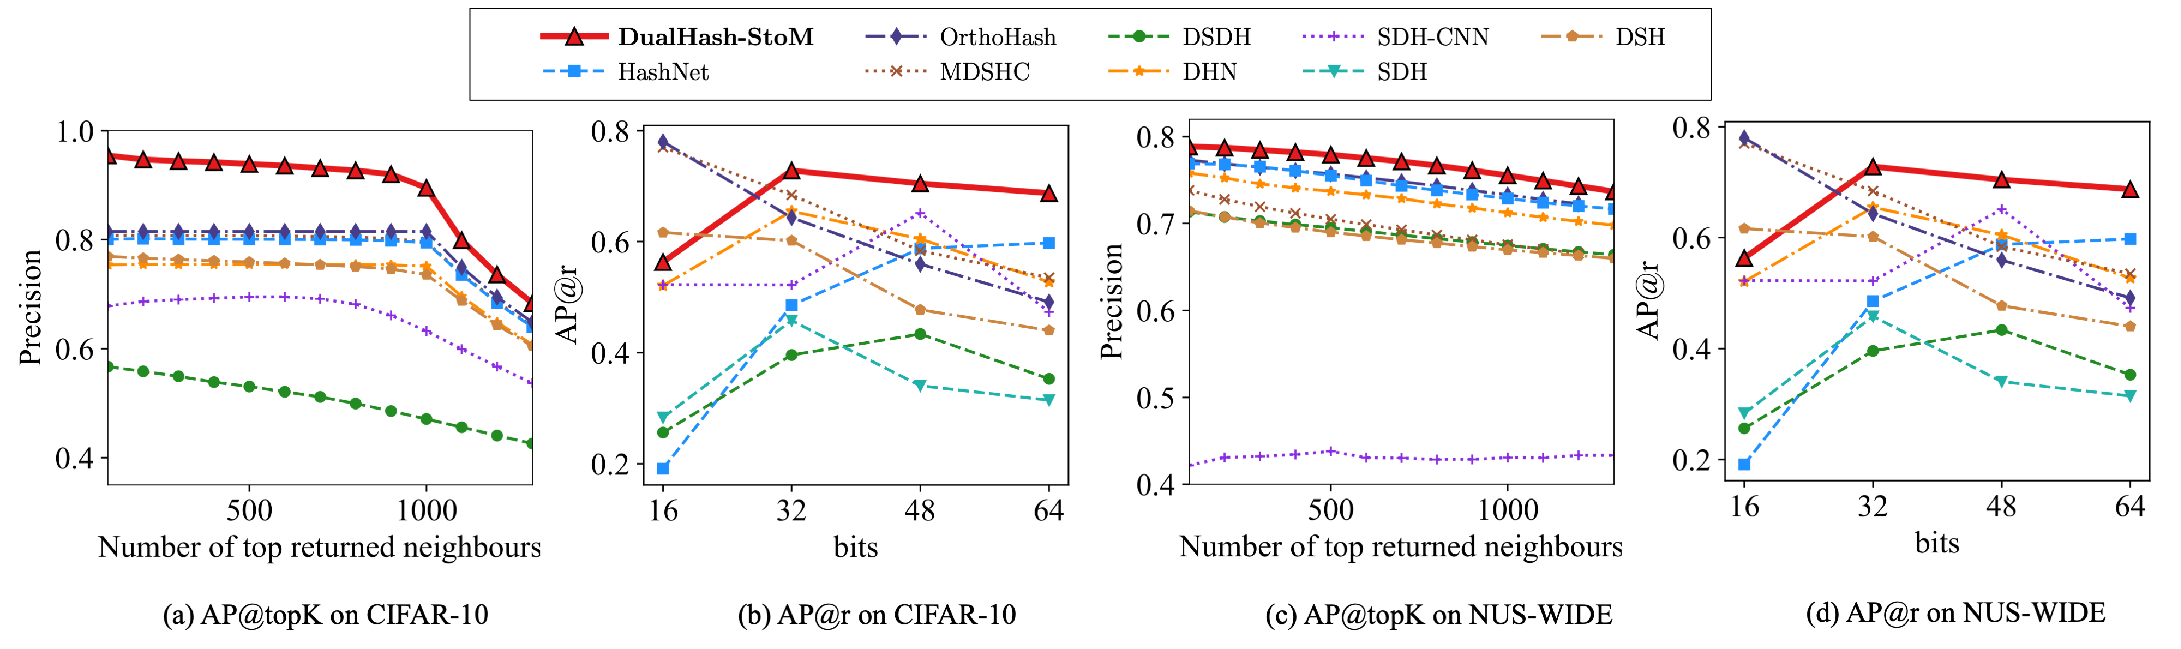
\includegraphics[width=0.95\linewidth]{results_images/ex2_4figures.pdf}
    \caption{Retrieval performance of DualHash and baselines on CIFAR-10 and NUS-WIDE datasets. (a), (c): P@topK with 64 bits;  (b), (d): P@r(=2) with different numbers of bits.}
 \label{fig:retrieval_2datasets}
    \vspace{-2ex}
\end{figure}
\begin{table}[t]
    \centering
    \caption{The mAP results of DualHash and baselines with different numbers of bits on CIFAR-10 and NUS-WIDE datasets with ResNet50 backbone.}
    \label{Table: performance_comparison_resnet50_small}
    \resizebox{\linewidth}{!}{
    \begin{tabular}{ccccccccc}
        \toprule
         & \multicolumn{4}{c}{CIFAR-10 (mAP@All)} & \multicolumn{4}{c}{NUS-WIDE (mAP@5000)} \\
        \cmidrule(lr){2-5} \cmidrule(lr){6-9}
         Method (ResNet50) & 16 bits & 32 bits & 48 bits & 64 bits & 16 bits & 32 bits & 48 bits & 64 bits \\
        \midrule
        DSH \cite{liuDeepSupervisedHashing} & 0.7403 & 0.8116 & 0.8217 & 0.8239 & 0.5559 & 0.6952 & 0.6981 & 0.7165 \\
        OrthoHash \cite{hoeOneLossAll2021} & \textbf{0.9032} & 0.9182 & 0.9202 & 0.9224 & \textbf{0.7448} & 0.7600 & 0.7569 & 0.7863 \\
        MDSHC \cite{wang2023deep} & 0.8980 & 0.9007 & 0.9063 & 0.9227 & 0.6428 & 0.7002 & 0.7248 & 0.7758 \\
        \cmidrule(lr){2-9}
        DualHash-StoM & 0.8559 & \textbf{0.9202} & \textbf{0.9392} & \textbf{0.9416} & 0.6538 & \textbf{0.7783} & \textbf{0.7721} & \textbf{0.8016} \\
        \bottomrule
    \end{tabular}}
    \vspace{2ex}
    \parbox{\linewidth}{\footnotesize
    \textbf{Bold} values indicate the best results.
    }
    \vspace{-1ex}
\end{table}
We provide empirical evidence that is consistent with our theoretical results (Theorems \ref{Theorem: the oracle complexity in SGDM} and \ref{Theorem: the oracle complexity in STORM}) and compare with HashNet, OrthoHash, and MDSHC with 64 bits on CIFAR-10 and NUS-WIDE. 
\Cref{fig:training_loss_map_2datasets} shows the training loss and validation mAP curves over epochs.
As shown in \Cref{fig:training_loss_map_2datasets} (a)-(b), DualHash-StoRM achieves the fastest convergence and lowest loss values on CIFAR-10 and NUS-WIDE, requiring only approximately 25 epochs on CIFAR-10. This aligns with our theoretical outcome: the variance reduction mechanism accelerates convergence. Though slower than DualHash-StoRM, DualHash-StoM still outperforms other baselines (approximately 75 epochs on CIFAR-10). 
Meanwhile, \Cref{fig:training_loss_map_2datasets} (c)-(d) show that although DualHash-StoRM converges faster during training, DualHash-StoM ultimately exhibits superior retrieval performance compared to other baselines. 
% \vspace{3pt}
\subsection{Comparison of Retrieval Performance}
\label{Subsection: Comparison of retrieval performance}
\begin{table}[t]
% \vspace{2ex}
    \centering
    \caption{The mAP results of DualHash and baselines with different numbers of bits on the ImageNet-100 dataset with ResNet50 backbone.}
    \label{tab:performance_imagenet_resnet50}
    \small
    \begin{tabular}{lcccc}
     \toprule
 & \multicolumn{4}{c}{ImageNet-100 (mAP@1000)} \\
\cmidrule(lr){2-5}
Method (ResNet50) & 16 bits & 32 bits & 48 bits & 64 bits \\
\midrule
DSH \cite{liuDeepSupervisedHashing} & 0.7179 & 0.7448 & 0.7335 & 0.7585 \\
OrthoHash \cite{hoeOneLossAll2021} & 0.8040 & \textbf{0.8292} & 0.8510 & 0.8636 \\
MDSHC \cite{wang2023deep} & \textbf{0.8047} & 0.8131 & 0.8561 & 0.8657 \\
 \cmidrule(lr){2-5}
DualHash-StoM & 0.7402 & 0.7705 & \textbf{0.8662} & \textbf{0.8714} \\
        \bottomrule
    \end{tabular}
    \vspace{2ex}
    \parbox{\linewidth}{\footnotesize
    \textbf{Bold} values indicate the best results.
    }
    \vspace{-2ex}
\end{table}
We report retrieval performance on CIFAR-10 and NUS-WIDE datasets, as shown in Table \ref{Table: baselines mAP}
% , \ref{Table: performance_comparison_resnet50_small}, \ref{tab:performance_imagenet_resnet50} 
and \Cref{fig:retrieval_2datasets}. 
In terms of mAP, DualHash methods consistently outperform most baselines, including recent advanced methods like OrthoHash and MDSHC.
On CIFAR-10, DualHash-StoM achieves 0.8539 mAP with 64 bits, outperforming OrthoHash (0.8355). On the NUS-WIDE dataset, it reaches 0.7448 mAP, significantly superior to MDSHC (0.6493).  
Although slightly less accurate than the StoM variant, DualHash-StoRM remains comparable to other baselines, providing a trade-off between accuracy and efficiency. 

To further demonstrate the scalability of our approach, we evaluate our method and three baselines using a \textbf{ResNet50 backbone}. As shown in \Cref{Table: performance_comparison_resnet50_small}, this modern architecture brings substantial performance gains in terms of mAP for all methods across CIFAR-10 and NUS-WIDE. Our DualHash-StoM, for example, achieves mAP improvements of 10.3\% on CIFAR-10 (0.9416 vs 0.8539) and 7.6\% on NUS-WIDE (0.8016 vs 0.7448) at 64 bits. Nevertheless, our method consistently maintains peak performance at 32 bits or more, outperforming all baseline methods. Moreover, on the more complex ImageNet-100 dataset, our method continues to demonstrate superior performance. As reported in \Cref{tab:performance_imagenet_resnet50}, DualHash-StoM reaches 86.62\% and 87.14\% mAP at 48 and 64 bits, outperforming all baselines. These results confirm that our method maintains robust performance and strong generalization capability as data complexity increases.

For P@topK (\Cref{fig:retrieval_2datasets} (a),(c)),  DualHash maintains 0.9 precision at lower top-k values on CIFAR-10, significantly outperforming other methods. This indicates that our method is suitable for precision-oriented image retrieval systems.
For P@r=2 (\Cref{fig:retrieval_2datasets} (b),(d)), DualHash-StoM consistently maintains peak performance at 32 bits and above, with 32 bits being optimal across CIFAR-10 and NUS-WIDE. These results align with the fact that as bit length increases, the Hamming space becomes sparse and few data points fall within the Hamming ball with radius 2 \cite{norouzi2012fast}.
% \vspace{3pt}

\subsection{Quantization Error Analysis}
\label{Subsection: Further analysis}
\begin{figure}[t]
% \vspace{-2ex}
    \centering
    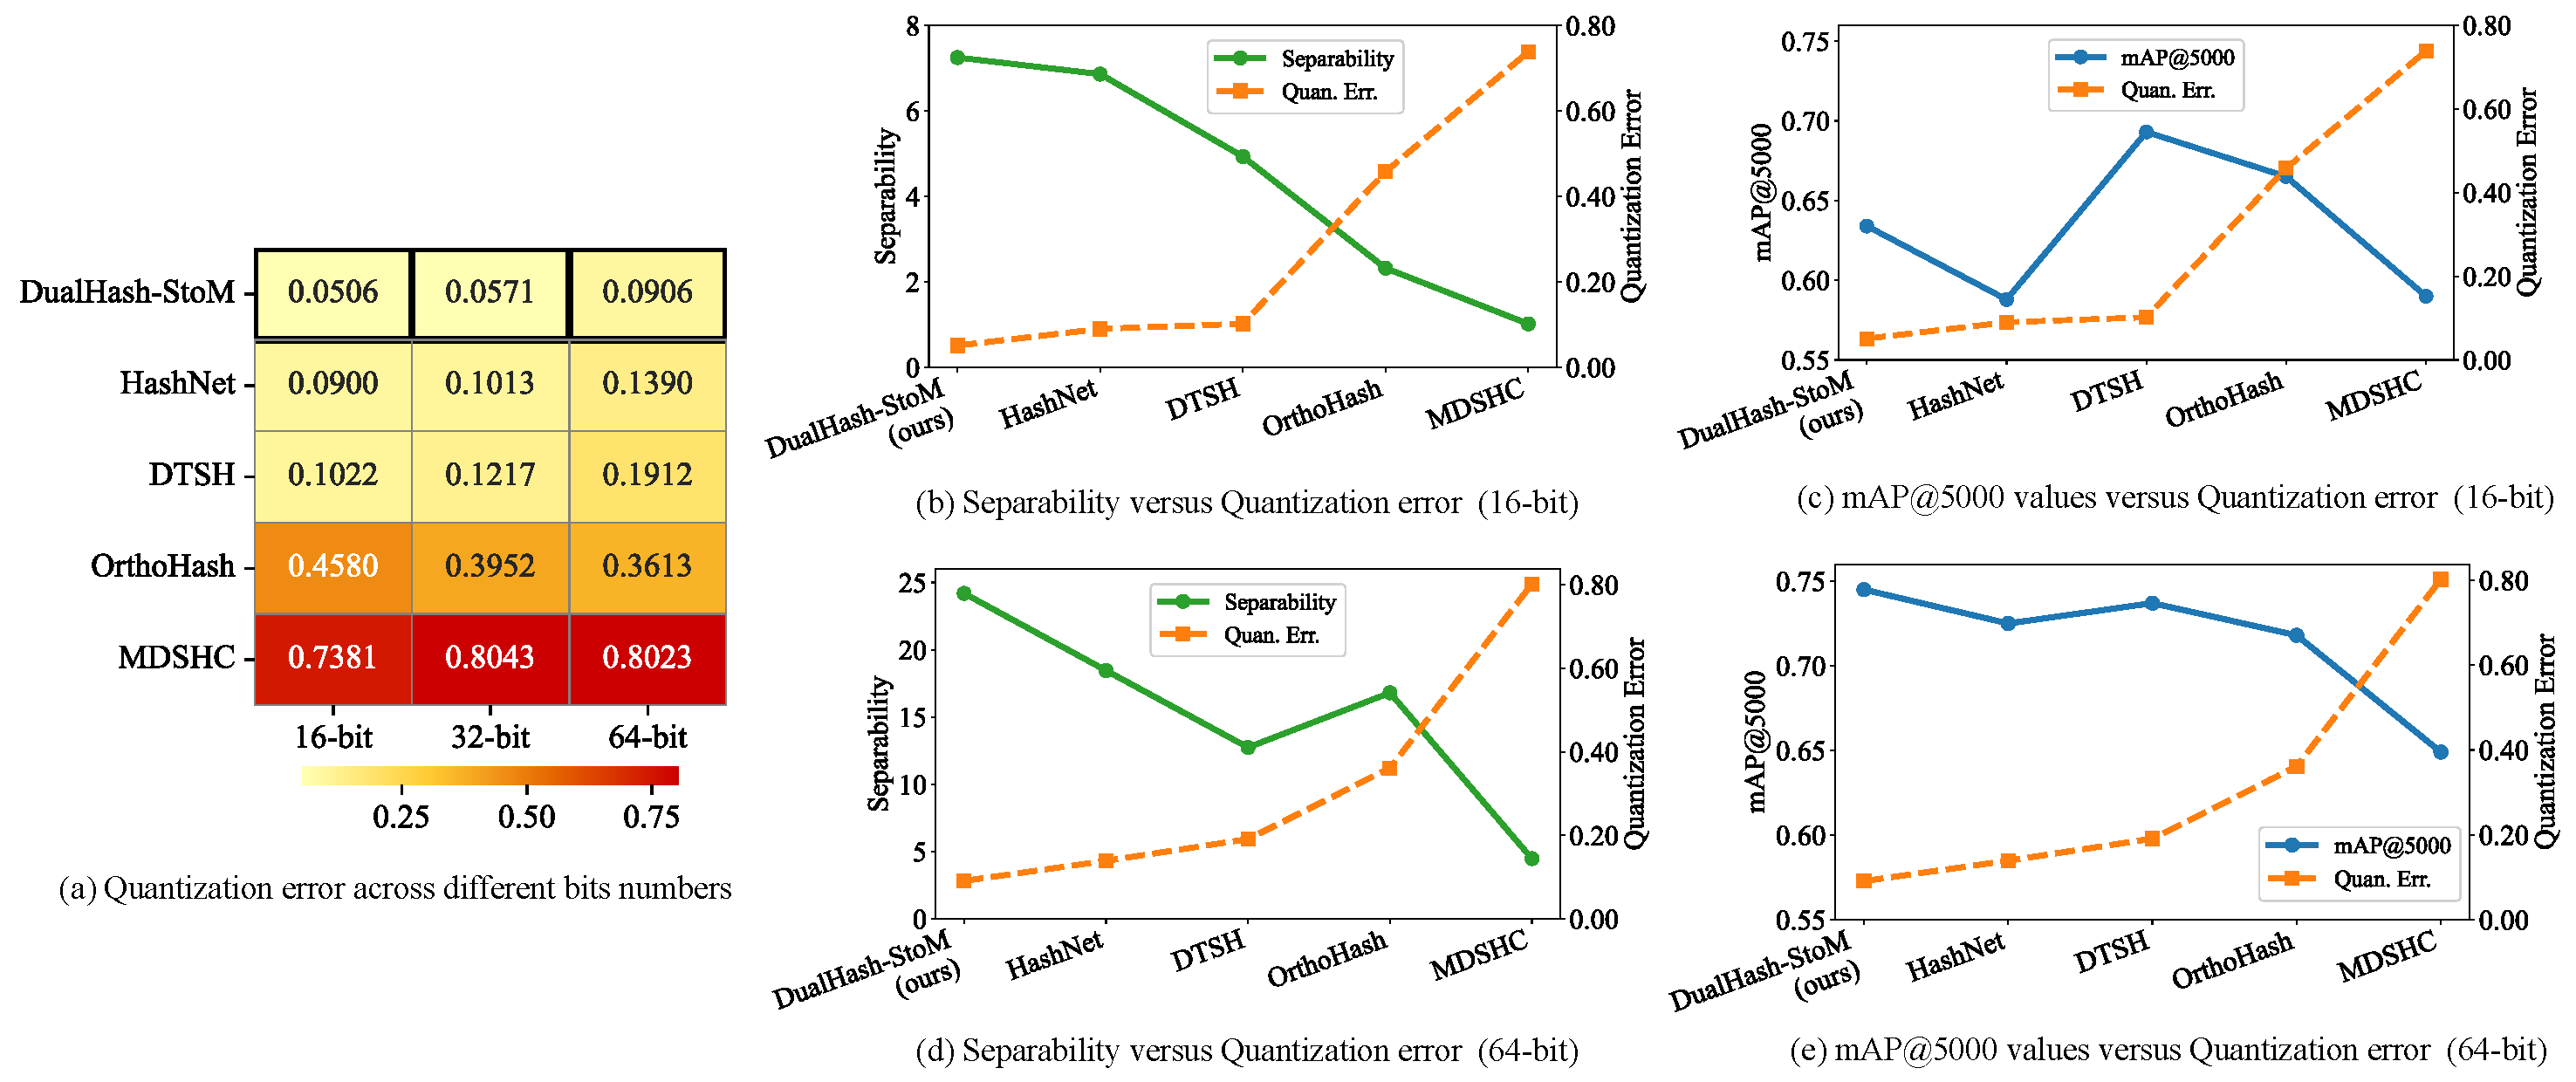
\includegraphics[width=0.95\linewidth]{results_images/quantization_error_further_analysis.pdf}
    \caption{Quantization error and its impact on retrieval performance across different numbers of bits on  NUS-WIDE.}
    \label{fig:quantization_error}
\end{figure}
\begin{figure}[t]
    \vspace{-2ex}
    \centering
    \includegraphics[width=0.95\linewidth]{results_images/hamming_hig_64.pdf}
    \caption{Histogram of intra-class and inter-class Hamming distances of DualHash and baselines with 64 bits on the NUS-WIDE dataset. The arrow annotation is the separability in Hamming distances, \(\EE [D_{inter}] - \EE [D_{intra}]\). We normalized the frequency so that the sum of all bins equals to 1.}
    \label{fig: His_64_NUSWIDE}
    \vspace{-2ex}
\end{figure}
\begin{figure}[t]
    \vspace{-2ex}
    \centering
    \includegraphics[width=0.95\linewidth]{results_images/hamming_hig_16.pdf}
    \caption{Histogram of intra-class and inter-class Hamming distances of DualHash and baselines with 16 bits on NUS-WIDE.}
    \label{fig: His_16_NUSWIDE}
    \vspace{-2ex}
\end{figure}
\begin{figure}[t]
    % \vspace{-1mm}
    \centering
    \includegraphics[width=0.95\linewidth]{results_images/sensitivity_2datasets.pdf}
    \caption{The mAP results of DualHash-StoM with Different settings of \(\eta\) and \(\lambda\) with 64 \& 16 bits on CIFAR-10 and NUS-WIDE.}
    \label{fig: sensitivity analysis of DualHash}
    \vspace{-2ex}
\end{figure}
To elucidate the mechanisms behind the performance of DualHash, following \cite{hoeOneLossAll2021},
we examine the quantization error (the discrepancy between continuous outputs and binary codes, \Cref{fig:quantization_error}) and the Hamming distance distributions of the resulting hash codes (\Cref{fig: His_64_NUSWIDE,fig: His_16_NUSWIDE}) across different bit lengths $K$ on the NUS-WIDE dataset. We compare DualHash-StoM against four deep hashing methods: HashNet \cite{Cao2017HashNetDL} and OrthoHash \cite{hoeOneLossAll2021} (employing distinct quantization strategies), and DTSH \cite{wang2016DTSH} and MDSHC \cite{wang2023deep} (both utilizing $W$-type regularization).

\vspace{3pt}
\noindent\textbf{Quantization Error Correlates with Intra- and Inter-class Distances.}
We find that methods achieving smaller quantization errors produce hash codes with reduced intra-class distances and enhanced inter-class separability, as shown in \Cref{fig:quantization_error}(a) and \Cref{fig: His_16_NUSWIDE,fig: His_64_NUSWIDE}. In the 64-bit setting (\Cref{fig: His_64_NUSWIDE}), both HashNet and DualHash exhibit similar inter-class distributions (close to Hamming distance $K/2 = 32$). However, DualHash's lower quantization error (0.0906 vs. 0.1390) enables significantly superior separability, i.e., the difference in the mean of intra-class distance (the blue dotted line)
with the mean of inter-class distance (the orange dotted line). In contrast, MDSHC's high quantization error (0.8023) leads to substantially larger intra-class distances and weaker inter-class separation, yielding a $5\times$ inferior separability ratio (24.19 vs. 4.47). 
This demonstrates that reducing quantization error enhances code quality primarily by compressing intra-class distributions.

\vspace{3pt}
\noindent\textbf{DualHash Achieves Lower Quantization Error via Dual-Space Reformulation.}
As shown in \Cref{fig:quantization_error}(a), DualHash attains the smallest quantization error across different bit lengths among all evaluated methods. This performance advantage stems from a fundamental methodological innovation: DualHash employs a novel dual-space reformulation of the W-regularization. The convexity property inherent in our dual formulation's conjugate function yields significant optimization advantages compared to directly optimizing the original nonconvex regularization or activation functions. 

\vspace{3pt}
\noindent\textbf{Bit-Dependent Performance and the Separability-Semantics Trade-off.}
While lower quantization error generally improves separability (\Cref{fig:quantization_error}(b) and (d)), its impact on retrieval performance varies significantly across bit settings, revealing a fundamental trade-off between class separability and semantic preservation.

\noindent\textit{High-bit regime ($K = 64$): Lower quantization error helps produce high mAP.}
At $K = 64$ (Figures \ref{fig:quantization_error}(d) and (e)), lower quantization error consistently correlates with higher mAP by enhancing separability and preserving both semantic discriminability and visual feature quality. Methods achieving low quantization loss (e.g., DualHash, HashNet, and DTSH) demonstrate superior retrieval accuracy, with DualHash achieving peak mAP performance.

\noindent\textit{Low-bit regime ($K = 16$): Low quantization error may produce low performance.}
At $K = 16$ (\Cref{fig:quantization_error}(b) and (c)), we observe a contrasting pattern: both extremely low and extremely high quantization error methods yield suboptimal performance. Notably, DTSH, which maintains intermediate quantization error, achieves superior mAP. Methods with very low quantization error (e.g., DualHash and HashNet) exhibit relatively lower mAP, particularly on multi-label datasets (e.g., NUS-WIDE). Specifically, we observe that  DualHash generates hash codes with low intra-class distances and high inter-class separation. This creates relatively clean class separation, but the actual visual relationships between images may get lost. Consequently, DualHash excels on simple datasets like CIFAR-10 but shows relatively lower performance on complex datasets like NUS-WIDE (multi-label) and ImageNet-100 (large-scale single-label).

% \vspace{3pt}
\subsection{Parameter Sensitivity Analysis}
To explore the sensitivity of key hyperparameters $\eta$ and $\lambda$ in 
DualHash, we conduct a grid search with $\eta \in \{10^{-4}, 10^{-3}, 
10^{-2}, 10^{-1}\}$ and $\lambda \in \{10^{-3}, 10^{-2}, 5\times 10^{-2}, 10^{-1}\}$. Unlike many deep hashing 
methods that exhibit significant hyperparameter sensitivity, DualHash-StoM 
demonstrates robust performance across a wide range of hyperparameter 
combinations (see \Cref{fig: sensitivity analysis of DualHash}). 
Specifically, 64-bit codes achieve excellent stability with mAP variations 
below 3\% on CIFAR-10 and 8\% on NUS-WIDE. While 16-bit codes show greater 
sensitivity (up to 18\% on CIFAR-10), this behavior is consistent with the 
intrinsic optimization challenges of extremely compact hash codes. Overall, 
the method demonstrates strong stability for standard hash lengths ($\geq$64 bits), 
which simplifies hyperparameter tuning in practical high-precision retrieval 
applications.
